\chapter{Description du capteur}\label{ch:capteur}

Le travail du capteur et d'acquérir les données nécessaires, puis de les transmettre à intervalles réguliers par la couche radio LoRa à la passerelle. Le cœur du capteur est le micro-contrôleur, celui-ci permet l'exécution du firmware qui est en charge de la gestion des opérations. C'est cette application qui va effectuer aux moments voulus les acquisitions nécessaire et ensuite créer un paquet de données pour être  envoyé.

Pour se faire le capteur est munit de plusieurs modules permettant l'acquisition des différents paramètres. Il sont présentés dans la liste suivante.

\begin{itemize}
\item GPS: Il permettra de connaître la position (latitude/longitude) du capteur et également d'avoir une référence de temps. Voir la section \ref{ch:module_ubloxeva8m} pour plus de détails.
\item Accéléromètre: Ce module sera utilisé pour connaître le nombre de pas effectués par le sportif ce qui permettra de calculer sa cadence de course. Voir la section \ref{ch:module_lsm303agr} pour plus de détails.
\item Rythme cardiaque:  Au moyen d'une sangle pectorale portée par l'athlète, ce module déclenchera une impulsion à chaque fois qu'un battement du cœur sera détecté. Voir la section \ref{ch:module_hr} pour plus de détails.
\item Radio LoRa: C'est au moyen de cet élément que le capteur transmettra les paquets de données à la passerelle. Voir la section \ref{ch:module_rn2483} pour plus de détails.
\end{itemize}

Dans le cadre du travail de Bachelor, un seul exemplaire de capteur sera assemblé et utilisé durant les tests.

\subsection{Les contraintes}

Le capteur est également soumis à des contraintes liées à son utilisation dans les conditions d'une compétition sportive.

Afin de gêner au minimum le sportif pendant la course et afin que le capteur soit utilisable pour l'entièreté d'une compétition, il est soumis aux contraintes définit durant la pré-étude et listé ci-dessous.

\begin{itemize}
\item Veiller à ce que sa taille soit minimale
\item Son poids ne doit pas dépasser 200 g
\item Il doit disposer d'une autonomie d'au moins 10 heures
\item Il doit être capable de transmettre les paquets de données à une passerelle située à une distance de 5 km en espace libre
\item Il sera placé dans un boîtier étanche
\end{itemize}

\section{Le matériel}

Lors de la pré-étude du projet, trois différentes cartes avaient été étudiée chacune avec leurs avantages et inconvénients. Pour la réalisation du projet, j'ai décidé d'utiliser la carte qui dispose de base du plus de module, c'est à dire la carte SODAQ One. En effet elle a l'immense avantage d'embarquer de base un module LoRa, un module GPS ainsi qu'un accéléromètre ce qui me permet de me focaliser sur le développement du logiciel embarqué. Il reste seulement à connecter sur une entrée du micro-contrôleur le module qui permettra de compter les battements du cœur en détectant les impulsions produite. Enfin afin de faciliter le debug de l'application embarquée, un UART et une sonde de debug seront également connectés pendant la phase de debug ce qui permettra d'afficher des messages et de permettre le debug du firmware. Un autre avantage de taille est que son micro-contrôleur est déjà disponible dans le système d'exploitation Zephyr ce qui facilitera le travail de portage.

Pour rappel, les caractéristiques du SODAQ One sont décrit dans la table~\ref{tab:sodaq_one_cara}.

\begin{table}[htb]
\caption[Caractéristiques de la carte SODAQ One v3]{Caractéristiques de la carte SODAQ One v3}
\label{tab:sodaq_one_cara}
\centering
\begin{tabular}{ l | l }
\toprule
Dimensions & 45mm x 25mm \\
\midrule
Microcontrôleur & ATSAMD21G18 – ARM Cortex M0 \\
\midrule
Oscillateur & 48 Mhz \\
\midrule
Flash & 256 kB \\
\midrule
RAM & 32 kB \\
\midrule
LoRa & Microchip RN2483 \\
\midrule
GPS & uBlox EVA 8M \\
\midrule
Accéléromètre & STMicroelectronics LSM303AGR \\
\midrule
Prix & 114 CHF\\
\bottomrule 
\end{tabular}
\end{table}

Aux modules de base, comme expliqué précédemment, il faudra rajouter un module qui permettra de compter le nombre de battement du cœur. Il est développé par la société Adafruit sous le nom de "Adafruit Heart Rate Start Pack".

\todo{PHOTO SODAQ}

Le module LoRa RN2483 est connecté par un lien série UART et utilise une interface de type AT commands, c'est à dire qu'il est piloté avec l'envoie de chaînes de caractère représentant des commandes, dans la même idée les réponses reçues sont de type text. Le module GPS ainsi que l'accéléromètre sont quant à eux connecté sur le bus $I^{2}C$. Le module rythme cardiaque sera lui connecté simplement sur un General Purpose I/O.

Le schéma block~\ref{fig:schema_block_sodaq} présente les différents modules et leurs connections avec le micro-contrôleur.

\todo{Ajouter debug SEGGER}

\begin{figure}[htb]
\centering 
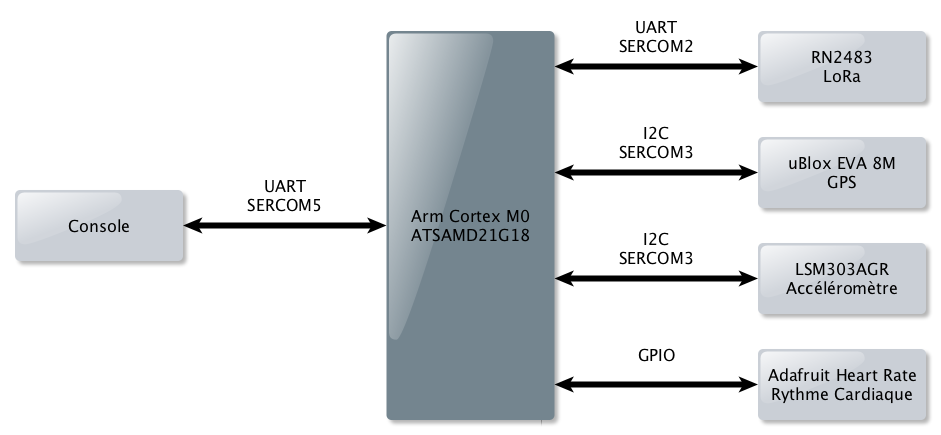
\includegraphics[width=1\columnwidth]{sensor_schema.png} 
\caption{Schéma block du capteur SODAQ One}
\label{fig:schema_block_sodaq}
\end{figure}

\subsection{Le module GPS UBloxEVA8M}\label{ch:module_ubloxeva8m}

\todo{figure}

Le EVA8M de la compagnie UBlox est un module GPS à haute précision et qui propose 8 moteurs de positionnement avec des performances très intéressantes. Il est capable de gérer les signaux GPS, GLONASS, QZSS et SBAS et dispose d'une sensibilité très haute de -164 dBm. Son temps d'acquisition de la position est minime et il dispose de mécanisme d'optimisation de la consommation d'énergie.

Ce module est très simple d'utilisation, dispose de son propre oscillateur et pour la plupart des applications il ne requiert qu'une antenne GNSS externe. De plus il propose plusieurs interfaces différentes, SPI, USB, $I^{2}C$ et UART.

Il assure une précision de la position GPS à 2.5 m et de 4 m en GLONASS, Il est capable de générer des messages jusqu'à une fréquence de 18 Hz et il propose 3 protocoles différents, NMEA, UBX et RTCM.

Une fois le module configuré par l'utilisateur, il va générer les messages voulues à une certaine fréquence. En fonction des message différentes information seront disponible, le choix des messages sélectionnés dépend du type d'application que l'on souhaite réaliser. Lorsque la configuration est effectuée, il suffit à l'utilisateur de venir lire la queue de message du module périodiquement afin de pouvoir y récupérer les messages et d'y extraire les informations.

Le module est détaillé dans le datasheet \cite{ublox-datasheet} ainsi que dans le document d'explication de son protocole \cite{ublox-protocol}.

\subsection{Le module LoRa RN2483}\label{ch:module_rn2483}

\todo{figure}

Le RN2483 est un module de gestion de la couche radio LoRa et également de la couche protocolaire LoRaWAN. Il utilise un simple protocole de commande/réponse sur une interface de type UART. Bien qu'il ne soit pas utilisé dans ce projet, le module est capable d'assurer la gestion de la couche LoRaWAN de classe A automatiquement, c'est à dire de la gestion du mécanisme d'authentification avec gestion du chiffrement des messages LoRa et du reste des mécanismes propres au LoRaWAN.

Chose intéressante, il est possible de désactiver entièrement la couche protocolaire LoRaWAN si l'on désire uniquement utiliser la couche radio LoRa, ce qui est le cas de ce projet. Dans ce cas de figure tous les éléments de gestion du protocole sont désactivés, reste la possibilité de configurer la couche radio LoRa avec la modification des différents paramètres, comme le facteur d'étalement ou la puissance de sortie du signal par exemple, et l'envoie ou la réception de données.

En plus le composant est capable d'envoyer les signaux en utilisant diverses modulations, FSK, GFSK ou LoRa.

L'utilisation ainsi que toutes les commandes sont décrite dans la datasheet du composant \cite{rn2483-datasheet}.

\subsection{Le module rythme cardiaque Adafruit}\label{ch:module_hr}

Le module Adafruit pour le rythme cardiaque est composé de deux éléments principaux, d'une part la sangle pectorale qui sera portée par le sportif et le récepteur qui permettra au micro-contrôleur de détecter les battements du cœur. La sangle et le récepteur utilise le protocole sans-fil WeakLink+ de la compagnie Polar ce qui permet au récepteur, lorsqu'un battement est transmis par la sangle, de générer une impulsion sur une entrée du micro-contrôleur. Cette impulsion est détectée par le micro-contrôleur grâce au driver External Interrupt Controller spécialement développé pour ce projet et qui permet de déclencher des interruptions lors de la détection d'un flanc montant par exemple.

\todo{figure}

\subsection{Le module accéléromètre LSM303AGR}\label{ch:module_lsm303agr}

\todo{figure}

Le LSM303AGR est un accéléromètre trois axes couplé à un magnétomètre. Seul l'accéléromètre est utilisé dans le cadre du projet, il est utilisé afin de détecter lorsque le sportif effectue un pas. Le composant est capable de proposer des échelles d'accélération linéaire de +/-2 à +/-16g, il peut communiquer soit sur le bus $I^{2}C$, ce qui est le cas sur la carte SODAQ One mais il peut aussi être connecté à un bus SPI. Il propose toute une série de registres qui permettent de configurer les différents paramètres de l'accéléromètre ainsi que du magnétomètre et de récupérer les valeurs d'accélération sur chaque axes. Il est aussi possible de configurer l'utilisation d'une FIFO, auquel cas plusieurs valeurs d'accélérations peuvent être stockées à la suite et lues lorsque nécessaire.

Enfin le module peut être configuré pour générer une interruption lorsqu'un certain seuil d'accélération est dépassé sur une combinaison des 3 axes afin de pouvoir détecter un certain mouvement ou déplacement par exemple. 

\subsection{L'accumulateur}

\todo{figure}

L'accumulateur utilisé pour alimenter la carte SODAQ One est de type lithium-polymère, solution assurant une sécurité accrue mais distribuant un peu moins d'énergie qu'un accumulateur de type lithium-ion par exemple.

Cet accumulateur est capable de délivrer environ 3.7V et 1200 mAh.

\todo{Discharge figure?}

\section{Le système d'exploitation Zephyr}

Zephyr project ou Zephyr est un système d'exploitation temps réel (RTOS) open source réalisé par la Linux Foundation. Il a été développé pour être utilisé sur des petits systèmes embarqués avec de grosses contraintes au niveau des ressources à disposition. A sa base il reprend un "micro" noyau développé par la société Wind River pour son système d'exploitation commercial VxWorks qui est employé dans beaucoup de projet dans les domaines aérospatial, militaire et automobile.
Plusieurs architectures de micro-contrôleur sont pris en charge comme ARM, RISC ou x86 par exemple et plusieurs dizaines de configuration pour différentes cartes du marché existent. 

Ce RTOS est également très facile a configurer pour ses propres besoins au moyen de fichiers de configuration ou l'on peut sélectionner les éléments que l'on veut utiliser dans son application. De plus il propose toutes les fonctionnalités que l'on peut attendre de ce genre de système: scheduler, thread, semaphore, message queue, ring buffer, gestion de l'allocation de la mémoire dynamiquement...
En plus de ces fonctions de base il dispose également de drivers pour piloter différents types de composants comme des UART, SPI, ADC ou GPIO par exemple. Enfin des couches réseaux tel que Ethernet, IPv6 ou Bluetooth sont disponible ainsi que la gestion de système de fichier. \cite{zephyr_web}

Autour de cet RTOS Il existe une importante communauté qui travail activement sur son développement ce qui permet de pouvoir avoir des réponses à ses questions rapidement et efficacement.

Ce système d'exploitation a été choisi car en plus d'être moderne il dispose déjà de la configuration d'une carte très similaire au SODAQ One, le Adafruit Feather M0 Basic Proto qui embarque le même micro-contrôleur, ceci facilitera passablement le travail de modifications pour adapter la configuration du RTOS au SODAQ One. Cette configuration consiste a définir, grâce à des Device Tree, quels sont les composants que la carte embarque et sur quels ports ou pins ils sont connectés, cela permet ensuite au système d'exploitation de pouvoir les piloter correctement.

Même si beaucoup d'éléments sont déjà existant pour le micro-contrôleur utilisé par le SODAQ One, le développement d'un nouveau driver $I^{2}C$ ainsi qu'un driver de gestion des interruptions externes, ont été réalisés car il n'en n'existait aucun au moment ou j'ai commencé le travail de Bachelor. Le driver $I^{2}C$ est utilisé afin de pouvoir communiquer avec les modules GPS et accéléromètre. Le driver External Interrupt Controller est utilisé afin de détecter les battements du cœur, lors de cet événement une impulsion est générée par le module rythme cardiaque qui, grâce à ce driver, permet de déclencher une interruption. Les drivers développés dans le cadre du travail de diplôme sont décrit en détail dans la section \ref{ch:drivers}.

La figure \ref{fig:zephyr_archi} présente l'architecture du système d'exploitation temps-réel Zephyr.

\begin{figure}[htb]
\centering 
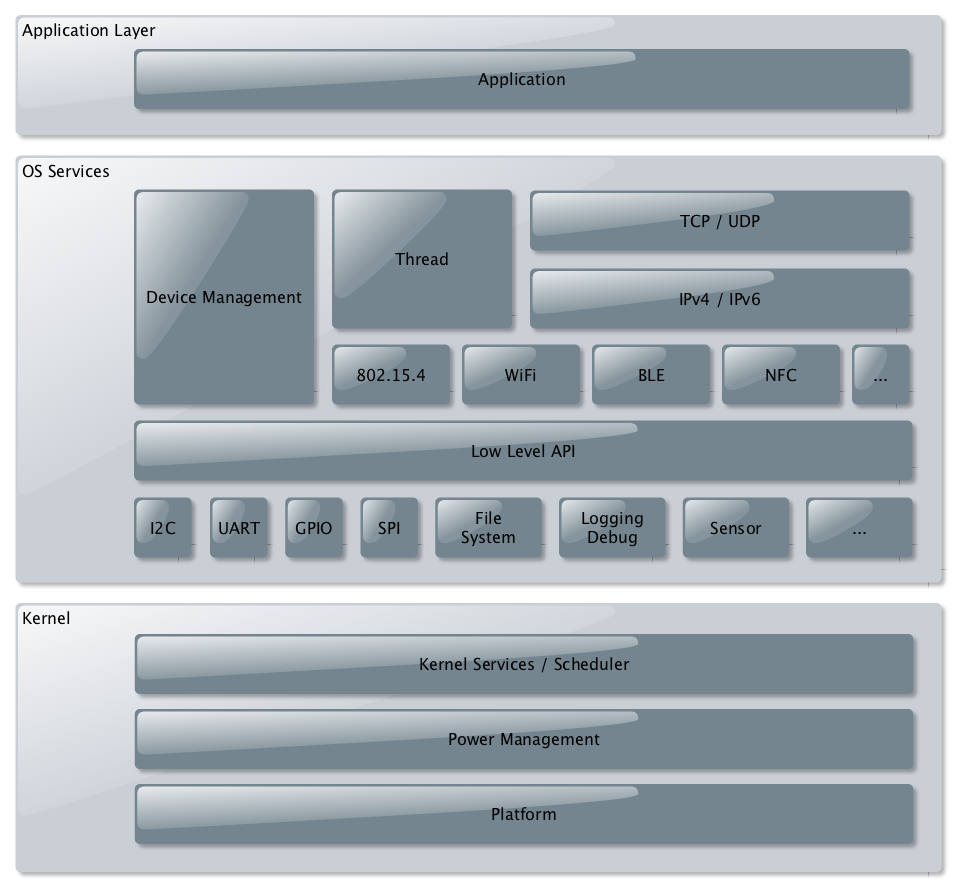
\includegraphics[width=1\columnwidth]{zephyr_archi.png} 
\caption{Architecture du système d'exploitation Zephyr - http://www.zephyrproject.org}
\label{fig:zephyr_archi}
\end{figure}

\subsection{Configuration Zephyr pour la carte SODAQ One}

Zephyr utilise un système de configuration qui permet de définir les périphériques qui sont présent sur une certaine carte. Cela permet ensuite aux utilisateurs de pouvoir accéder aux différents éléments grâce aux drivers proposés par le système d'exploitation. En plus de cela il est également nécessaire de configurer la fonction de chaque pins que l'on souhaite utiliser car elles ont souvent la possibilité d'en avoir plusieurs. Enfin l'on peut spécifier une configuration de base, par exemple en activant par défaut la gestion du bus $I^{2}C$.

Dans le cadre du projet, une nouvelle configuration a du être définit pour la carte SODAQ One.

Un fichier important est de type Device Tree (dts), c'est un type de fichier qui permet de définir avec des nœuds les composants disponibles. Les informations contenus dans ce fichier sont spécifiques à une certaine carte car elles dépendent de la façon dont les périphériques sont connectés au micro-contrôleur. Ce type de fichier est beaucoup utilisé par Linux par exemple.

Pour la carte SODAQ One, le fichier est principalement utilisé afin de définir le type de micro-contrôleur présent sur la carte ainsi que les composants SERCOM utilisés pour les divers périphérique. Enfin on peut spécifier quel composant doit être utilisé par Zephyr pour la console.

Un extrait de ce fichier est présenté ci-dessous.

\begin{lstlisting}
/*
 * Copyright (c) 2018 Leonard Bise
 *
 * SPDX-License-Identifier: Apache-2.0
 */

/dts-v1/;
#include <atmel/samd21.dtsi>

/ {
	model = "SODAQ One v3";
	compatible = "sodaq,one-v3", "atmel,samd21g18a",
			"atmel,samd21";

	chosen {
		zephyr,console = &sercom5;
		zephyr,sram = &sram0;
		zephyr,flash = &flash0;
		zephyr,code-partition = &code_partition;
	};
};

&sercom0 {
	status = "ok";
	compatible = "atmel,sam0-spi";
	#address-cells = <1>;
	#size-cells = <0>;
};

&sercom2 {
	status = "ok";
	compatible = "atmel,sam0-uart";
	current-speed = <57600>;
};

&sercom3 {
	status = "ok";
	compatible = "atmel,sam0-i2c";
	clock-frequency = <I2C_BITRATE_FAST>;	
};

&sercom5 {
	status = "ok";
	compatible = "atmel,sam0-uart";
	current-speed = <115200>;
};

...

\end{lstlisting}

\section{Le logiciel embarqué}

Cette section décrit le logiciel embarqué sur le capteur dans son ensemble. En se basant sur les fonctionnalités proposées par Zephyr ainsi que les drivers, qui sont décrit dans la section \ref{ch:drivers}, c'est lui qui va cadencer les acquisitions ainsi que l'envoie des paquets LoRa à la passerelle. Le logiciel embarqué ainsi que les drivers sont entièrement écrit en langage C. Il en va de même pour le système d'exploitation Zephyr qui contient cependant certaines parties écrites en assembleur.

La liste suivante présente toutes les acquisitions qui sont gérer par le logiciel.

\begin{itemize}
\item Position GPS message générer par le module à une fréquence de 1 Hz
\item Rythme cardiaque, une interruption est déclenchée à chaque battement du cœur
\item Comptage du nombre de pas, une interruption est déclenchée lorsqu'un pas est détecté par l'accéléromètre
\end{itemize}

De manière général et de façon simplifié on peut définir le processus du capteur comme dans la figure \ref{fig:sensor_process}.

\begin{figure}[htb]
\centering 
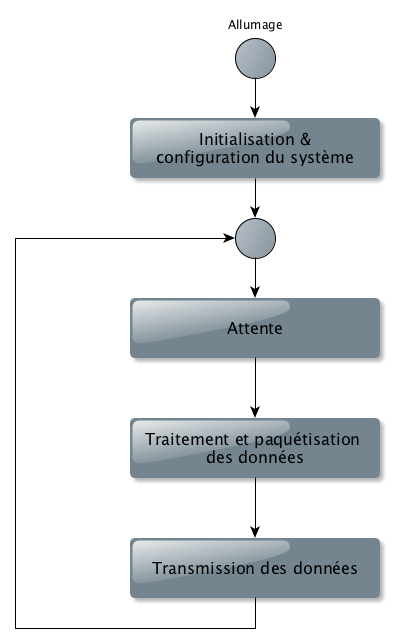
\includegraphics[width=0.5\columnwidth]{sensor_process.png} 
\caption{Processus général du capteur}
\label{fig:sensor_process}
\end{figure}

\subsection{Architecture logiciel}

La figure \ref{fig:sensor_static_archi} montre l'architecture statique du logiciel embarqué, tout les modules dont il est composé sont présentés.

\begin{figure}[htb]
\centering 
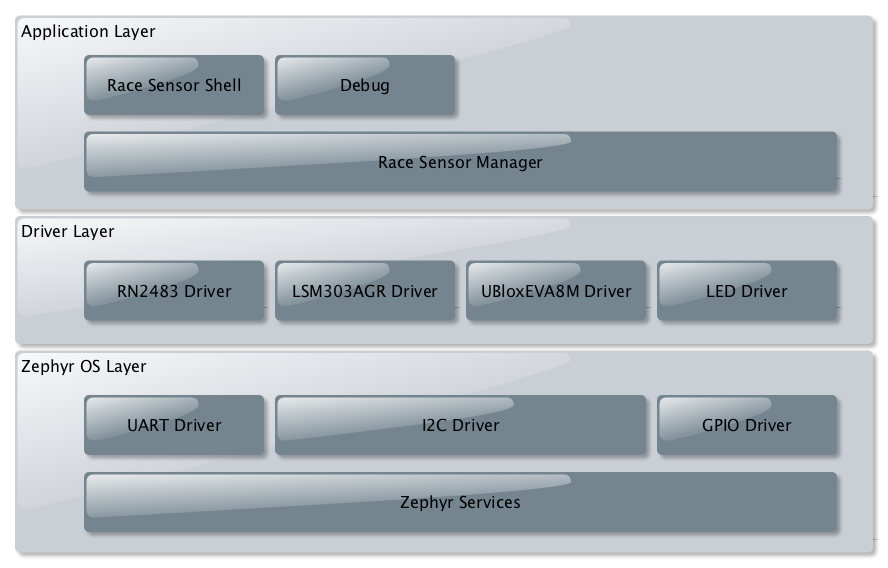
\includegraphics[width=1.0\columnwidth]{sensor_static_archi.png} 
\caption{Architecture statique du logiciel embarqué sur le capteur}
\label{fig:sensor_static_archi}
\end{figure}

Les éléments qui compose la couche application du logiciel embarqué sont décrit en plus de détail dans la liste ci-dessous.

\begin{itemize}
\item Race Sensor Manager: C'est le module responsable de la gestion du capteur, au moyen d'un thread c'est lui qui déclenche les acquisitions et qui paquetise les données afin de les transmettre dans des paquets LoRa.
\item Race Sensor Shell: Le shell du capteur, il est principalement utile pour les tests et le debug. Il propose plusieurs commande qui permettent par exemple de modifier la configuration de la liaison radio LoRa.
\item Debug: Ce module propose des fonctions qui facilite le debug de l'application.
\item Heart Rate: Compte le nombre de battement du cœur par unité de temps en s'appuyant sur l'accéléromètre Adafruit Heart Rate starter pack
\item Cadence: Permet le comptage des pas du sportifs par unité de temps grâce à l'accéléromètre LSM303AGR
\end{itemize}

La figure \ref{fig:sensor_dyn_archi} décrit les éléments dynamiques qui compose le logiciel du capteur.

\todo{Update when finished}

\begin{figure}[htb]
\centering 
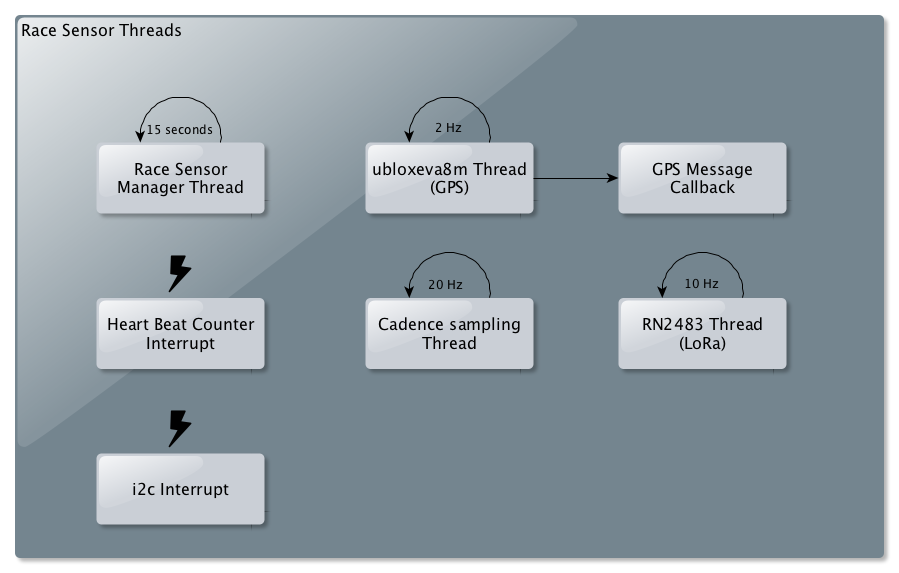
\includegraphics[width=1\columnwidth]{sensor_dyn_archi.png} 
\caption{Architecture dynamique du logiciel embarqué sur le capteur}
\label{fig:sensor_dyn_archi}
\end{figure}

\todo{Add missing thread frequencies}

Zephyr propose une implémentation de la priorité des threads intéressante qui permet en fonction de la valeur d'également modifier le comportement de l'ordonnanceur. La priorité d'un thread, valeur entière, peut être soit positive ou négative. Une valeur de priorité plus petite est plus importante qu'une valeur numériquement plus grande, ainsi un thread de priorité -2 est plus prioritaire qu'un de priorité 7.

En plus de cela, l'ordonnanceur distingue deux catégorie de thread en utilisant la valeur de priorité. Des threads dit coopératif et des threads pré-emptible.

Les threads coopératif ont une valeur de priorité négative, une fois qu'ils deviennent le thread exécutant, il le reste jusqu'à ce qu'il effectue une action qui le mettrait dans l'état non prêt, c'est à dire l'acquisition d'un sémaphore qui est utilisé ou une attente par exemple.

Un threads pré-emptible a une valeur de priorité non négative. Lors de son exécution ce genre de thread peut à tout moment être mis dans l'état non prêt par l'ordonnanceur afin de permettre à un thread coopératif ou à un thread pré-emptible de priorité plus haute ou égale de s'exécuter. \cite{zephyr_web}

La table \ref{tab:threads_cara} décrit en plus de détail les caractéristiques de chaque threads.

\begin{table}[htb]
\caption{Caractéristiques des threads du capteur}
\label{tab:threads_cara}
\centering
\begin{tabular}{ l l l }
\toprule
Thread & Priorité & Période \\
\midrule
Race Sensor Manager & Haute - 0 & 15 s  \\
RN2483 (LoRa) & 1 & 100 ms  \\
Driver UBloxEVA8M (GPS) & 2 & 100 ms  \\
Accéléromètre & Basse - 3 & 100 ms  \\
\bottomrule 
\end{tabular}
\end{table}

Le thread le plus prioritaire est celui du gestionnaire du capteur, en effet étant donné qu'il a une période qui est longue, lorsqu'il est prêt il doit directement prendre la main sur les autres threads afin de garantir la fréquence de transmission des données à la passerelle.
Le thread responsable de la transmission des données au module LoRa doit également faire son travail en priorité afin de garantir le transfert des données rapidement.
Enfin les thread de gestion du module GPS et de l'accéléromètre dispose de priorité plus faible car leur importance est moindre dans le processus du capteur.

\subsection{Race Sensor Manager}

Le Race Sensor Manager est le module principale du capteur, lors de l'allumage du capteur, c'est lui qui commence par configurer tous les éléments nécessaires au fonctionnement du capteur, comme les drivers par exemple. Une fois le système initialisé, le thread du Race Sensor Manager va s'occuper d'envoyer les données acquises dans des paquets LoRa à intervalle régulier.

La figure \ref{fig:race_sensor_manager_uml} présente le diagramme de classe du Race Sensor Manager.

\begin{figure}[htb]
\centering 
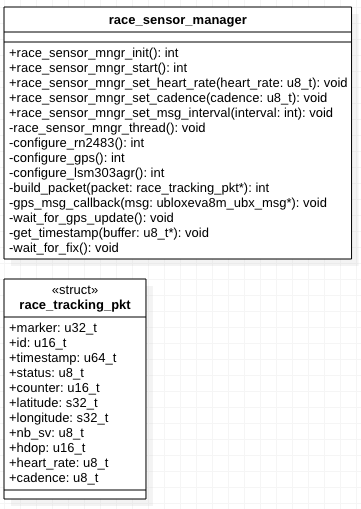
\includegraphics[width=0.5\columnwidth]{race_sensor_manager_uml.png} 
\caption{Diagramme de classe du Race Sensor Manager}
\label{fig:race_sensor_manager_uml}
\end{figure}

Lors du lancement du firmware du capteur, le Race Sensor Manager est initialisé puis lancé grâce aux fonctions \func{race\_sensor\_mngr\_init()} et \func{race\_sensor\_mngr\_start()}. Durant l'initialisation du module tous les drivers sont initialisé et les interfaces de communications sont configuré, au terme de cette opération le thread est lancé qui s'occupera du séquencement des opérations. Les opérations d'initialisation sont décrite dans le diagramme de séquence \ref{fig:race_sensor_manager_init_seq}.

\begin{figure}[htb]
\centering 
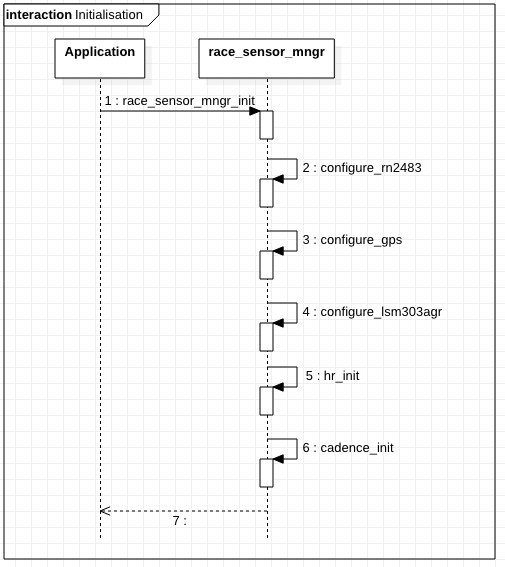
\includegraphics[width=0.7\columnwidth]{race_sensor_manager_seq_init.png} 
\caption{Diagramme de séquence de l'initialisation du Race Sensor Manager}
\label{fig:race_sensor_manager_init_seq}
\end{figure}

Le thread va s'occuper de paquetiser et d'envoyer les données collectées régulièrement, le comportement est décrit dans le digramme de séquence \ref{fig:race_sensor_manager_init_thread}.

\begin{figure}[htb]
\centering 
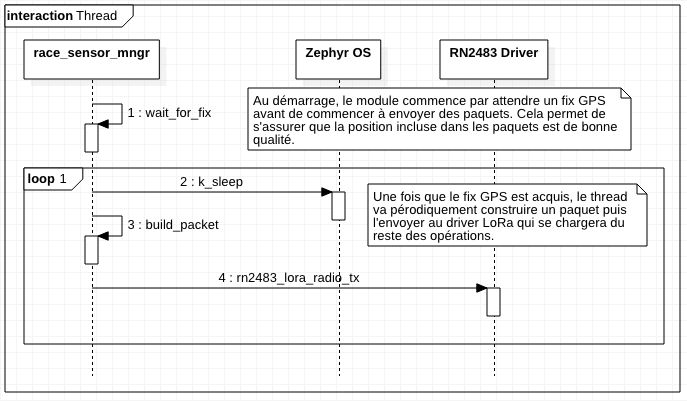
\includegraphics[width=1\columnwidth]{race_sensor_manager_seq_thread.png} 
\caption{Diagramme de séquence du thread du Race Sensor Manager}
\label{fig:race_sensor_manager_init_thread}
\end{figure}

\subsection{Heart Rate}

Le module Heart Rate est responsable de la gestion et du calcul du rythme cardiaque de l'athlète portant le capteur. Grâce au dispositif électronique permettant l'interfaçage avec la ceinture pectorale, ce module va placer une interruption, grâce au driver External Interrupt Controller et au driver GPIO de Zephyr, modifié pour l'occasion, sur la pin sur laquelle une impulsion est déclenchée lors d'un battement du cœur.  En mesurant le temps écoulé ainsi que le nombre de battement il est ensuite possible de calculer le rythme cardiaque qui est ensuite transmis dans les paquets à destination de la passerelle.

La figure \ref{fig:heartrate_uml} montre le diagramme de classe du module Heart Rate.

\begin{figure}[htb]
\centering 
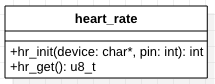
\includegraphics[width=0.3\columnwidth]{heartrate_uml.png} 
\caption{Diagrammede classe du module Heart Rate}
\label{fig:heartrate_uml}
\end{figure}

\subsection{Cadence}

\todo{Finish this}

La cadence du sportif est déterminé grâce à ce module. En se basant sur les données de l'accéléromètre, qui est capable de déterminer les accélérations sur les 3 axes x,y et z, il est possible de déterminer le moment ou un pas est effectué et donc de les compter. 

Afin de pouvoir facilement compter le nombre de pas, l'accéléromètre LSM303AGR est configuré en utilisant le système de seuil qu'il propose. Cela permet de déclencher des interruptions lorsqu'une accélération d'une certaine force est détecté sur les axes.

La figure \ref{fig:cadence_uml} montre le diagramme de classe du module Cadence.

\begin{figure}[htb]
\centering 
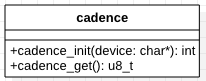
\includegraphics[width=0.3\columnwidth]{cadence_uml.png} 
\caption{Diagramme de classe du module Cadence}
\label{fig:cadence_uml}
\end{figure}

\subsection{Debug}

Ce module propose quelque fonction et macros qui sont utile pendant le debug du capteur comme l'affichage de message sur une console ou l'affichage de la liste de tous les threads qui sont actifs.

\subsection{Race Sensor Shell}

Le Race Sensor Shell permet l'utilisation d'un shell exécuté directement sur le capteur qui permet l'ajout de diverses commandes permettant la configuration du capteur pendant l'exécution du firmware. Il s'appuie sur le module shell proposé par Zephyr qui prend en charge la gestion du shell, il suffit de lui donner des pointeurs de fonction ainsi que des noms de fonction et le reste est pris en charge par le système d'exploitation.

La liste suivante montre les commandes disponible dans le shell du capteur:

\begin{itemize}
\item set\_lora\_sf: Permet de changer le facteur d'étalement de la couche radio LoRa
\item set\_lora\_pwr: Permet de changer la puissance de sortie du signal de la couche radio LoRa
\item set\_msg\_interval: Permet de modifier l'intervalle entre l'envoie de deux messages
\end{itemize}

\section{Les drivers}\label{ch:drivers}

Afin de pouvoir utiliser tous les modules requis par le projet ainsi que le RTOS Zephyr il a été nécessaire d'écrire plusieurs drivers qui sont décrits dans cette section.

Les drivers présenté dans la liste suivante ont été développés dans le cadre du travail de Bachelor.

\begin{itemize}
\item Driver $I^{2}C$ pour micro-contrôleur ATSAMD21G18 intégré au système d'exploitation Zephyr
\item Driver UBloxEVA8M pour piloter le module GPS qui se base lui même sur le driver $I^{2}C$
\item Driver LSM303AGR pour le module accéléromètre qui se base également sur le driver  $I^{2}C$
\item Driver RN2483 LoRa permettant d'exploiter la communication LoRa et qui se base sur le driver UART existant de Zephyr
\item Driver pour piloter les 3 LEDs de la carte SODAQ One au travers de GPIOs
\item Driver External Interrupt Controller permet de déclencher une interruption en fonction de l'état d'un I/O qui est utilisé pour pouvoir compter les battements du cœur
\end{itemize}

Enfin le Driver GPIO de Zephyr a du être modifié afin de pouvoir utiliser les interruptions sur les I/O proposés par le driver External Interrupt Controller.

\subsection{Driver $I^{2}C$ ATSAMD21G18}

$I^{2}C$ est un bus qui permet de connecter plusieurs esclaves à un maître. Le maître est le seul à initier les accès aux esclaves qui disposent chacun de leur adresse spécifique, lorsque le maître veut lire ou écrire sur un esclave il va envoyer un message $I^{2}C$ contenant l'adresse de l'esclave en question, suivi des données à écrire ou de l'adresse à lire par exemple. Avantage de taille est qu'il ne nécessite que deux connections pour fonctionner, une qui permet la distribution du signal de synchronisation qui est uniquement contrôlé par le maître et une autre pour le transfert des données qui peut être contrôlé soit par le maître lors d'une écriture ou de l'esclave pour une lecture.

L'écriture de ce driver se base sur les informations disponible dans la datasheet du micro-contrôleur ATSAMD21G18 \cite{samd21-datasheet}. Les composant SERCOM $I^{2}C$ sont décrit à partir de la page 545. L'application note \cite{samd21-i2c-configuration} a également été consultée.

\begin{figure}[htb]
\centering 
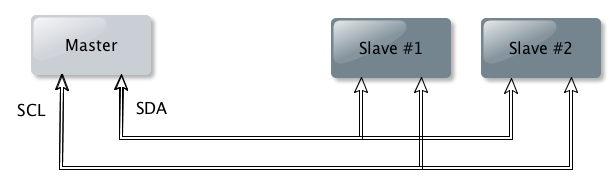
\includegraphics[width=0.8\columnwidth]{i2c_bus.png} 
\caption{Schéma d'un bus $I^{2}C$}
\label{fig:i2c_bus}
\end{figure}

Le bus $I^{2}C$ utilise un protocole pour la communication entre un maître et un esclave, en fonction de l'opération voulue le message ne sera pas tout à fait le même. Le maître commence toujours par envoyer un START suivi de l'adresse de l'esclave à qui est destiné le message et puis enfin du type d'opération, lecture ou écriture. Les données sont ensuite placé sur le bus par le maître dans le cas d'une écriture ou par l'esclave lors d'une lecture. Chose importante lorsque le maître à terminé le processus de lecture, il doit envoyé un message de type NACK suivi d'un STOP afin d'informer l'esclave de la fin du transfert.
La figure \ref{fig:i2c_messages} propose les deux types de messages qu'il existe.

\begin{figure}[htb]
\centering 
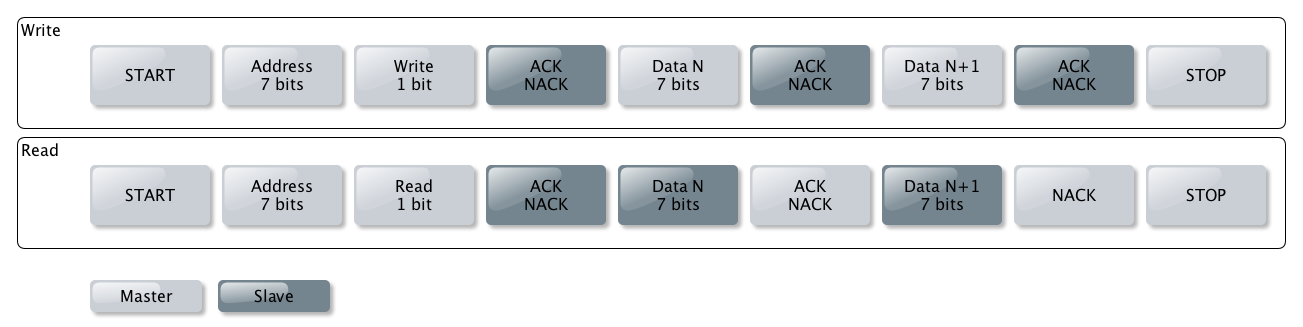
\includegraphics[width=1\columnwidth]{i2c_messages.png} 
\caption{Les messages $I^{2}C$}
\label{fig:i2c_messages}
\end{figure}

Le driver $I^{2}C$ est responsable du pilotage des SERCOM que propose le micro-contrôleur, ce sont des modules qui peuvent être configuré afin de proposer une interface de type UART, $I^{2}C$ ou SPI. Étant donné qu'il est intégré directement à Zephyr, il doit respecter les contraintes qui y sont liées c'est à dire d'être placé dans le dossier $I^{2}C$ du système d'exploitation: zephyr/drivers/i2c/i2c\_sam0.c et qu'il doit proposer une interface standardisée qui permet au système d'exploitation d'initier les opérations suivantes.

\begin{itemize}
\item Configuration de l'interface
\item Transfert de donnée (Lecture/Écriture)
\end{itemize}

Pour se faire, il faut remplir une structure avec des pointeurs de fonctions qui sont ensuite appelés par le système d'exploitation au besoin. En plus de cela, il faut définir et configurer un device, c'est la structure utilisée par Zephyr qui sera ensuite utilisée par les applications afin de pouvoir communiquer sur le bus $I^{2}C$.

C'est le driver qui en fonction de l'opération à effectuer va envoyer les codes (START ou STOP) suivie des données. Il produira les acquittement nécessaire et Il vérifiera également que l'esclave en question valide bien les messages. L'utilisation d'une l'interruption permet au driver de savoir, après avoir écrit un message dans le SERCOM, quand il a été effectivement envoyé ceci afin de pouvoir initier l'envoie du prochain message.

La figure \ref{fig:driver_i2c_uml} présente le diagramme de classe du driver $I^{2}C$.

\begin{figure}[htb]
\centering 
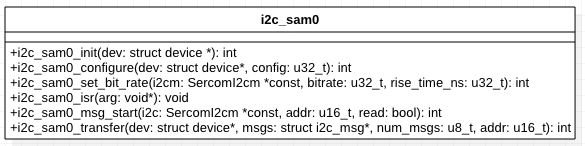
\includegraphics[width=0.8\columnwidth]{driver_i2c_uml.png} 
\caption{Diagramme de class du driver $I^{2}C$}
\label{fig:driver_i2c_uml}
\end{figure}

Un exemple d'utilisation du driver $I^{2}C$ est disponible ci-dessous.

\begin{lstlisting}[style=CStyle]
#include <i2c.h>

/* Address of the i2c slave */
#define I2C_DEVICE_ADDR 0x20

#define BUFFER_SIZE 128

void main(void) {
	/* Get binding on i2c device */
	struct device* i2c_dev = device_get_binding(CONFIG_I2C_SAM0_SERCOM3_LABEL);
	/* i2c device configuration */
	u32_t i2c_cfg = I2C_SPEED_SET(I2C_SPEED_FAST) | I2C_MODE_MASTER;
	uint8_t msg[BUFFER_SIZE];
	
	/* Check if binding succeeded */
	if (!i2c_dev) {
		DBG_PRINTK("%s: Binding to i2c failed\n", __func__);
		return;
	}
	/* Configure I2C Device */
	if (i2c_configure(i2c_dev, i2c_cfg)) {
		DBG_PRINTK("%s: i2c configuration failed\n", __func__);
		return;
	}	
	
	msg[0] = 0x11;
	msg[1] = 0x22;
	msg[2] = 0x33;
	msg[3] = 0x44;	
	
	/* Send message to i2c slave */
	if (i2c_write(i2c_dev, msg, 4, I2C_DEVICE_ADDR)) {
		DBG_PRINTK("%s: I2C access failed\n", __func__);
	}
	
	/* Read from i2c slave */
	if (i2c_read(i2c_dev, msg, 4, I2C_DEVICE_ADDR)) {
		DBG_PRINTK("%s: I2C access failed\n", __func__);
		return 0;
	}	
}
\end{lstlisting}

\subsection{Driver UBloxEVA8M}

Le driver UBloxEVA8M permet le pilotage du module GPS du même nom qui se trouve connecté sur le bus $I^{2}C$. Ce module est intégré directement à la carte SODAQ One et propose une gestion GPS complète, il est capable de recevoir les signaux GPS, GLONASS, QZSS et SBAS, il est extrêmement sensible, très rapide et de petite taille, en somme une solution idéal pour des capteurs de petite taille. Il est décrit en plus détails à la section \ref{ch:module_ubloxeva8m}. 

Le module utilise trois types de protocole pour la transmission des données et la configuration du module, NMEA, UPX et RTCM. NMEA est un protocole à base de texte qui envoie des messages formée de character ASCII il est idéale lorsque le module est connecté sur un UART. UPX est un protocole compact car il utilise des mots binaires qui sont protégés par des checksum. Enfin le protocole Radio Technical Commission for Maritime Services (RTCM) est unidirectionnel (seulement envoie vers le receveur) qui permet au receveur l'utilisation des corrections du positionnement relatif uniquement.
Le driver utilise les messages du protocole UPX car il est le mieux adapté pour l'utilisation sur un bus $I^{2}C$, il est décrit en détail dans le document \cite{ublox-protocol}.

Une fois que le module a été configuré, il va produire les messages qui ont été activés et contenant diverses informations et les placé dans une FIFO. Au travers du bus $I^{2}C$, le thread du driver va interroger le module périodiquement afin de savoir si des messages sont prêt à être lu, si c'est le cas le driver va lire les messages disponible et les stocker dans une structure de type ubloxeva8m\_ubx\_msg. L'utilisateur récupère les messages reçu grâce à une fonction callback qui est passée au driver et qu'il appelle à chaque fois qu'un message est prêt.

Dans le cadre du projet, le message UBX-NAV-PVT est utilisé pour récupérer les informations nécessaire au projet, c'est à dire la position, l'évaluation de la précision de la position ainsi que les informations de temps qui servent à synchroniser le capteur. La liste suivante présente un résumé des informations contenue dans ce message, pour plus de détails voir \cite[p.~307]{ublox-protocol}.

\begin{itemize}
 \item La date du jour
 \item L'heure actuelle 
 \item Le type de fix GPS
 \item La validité et la précision des informations contenus dans le message
 \item La latitude et longitude
 \item Le nombre de satellite actuellement vu
 \item La vitesse
 \end{itemize} 

En utilisant le driver $I^{2}C$ décrit à la section précédente il va permettre l'initialisation, la configuration et la récupération des messages GPS du composant. Une fois le module GPS initialisé et configuré, le driver utilise un thread qui va périodiquement allez voir si de nouveaux messages sont présent dans la FIFO, si c'est le cas ils sont lus et ensuite décodé. Lorsque les messages sont prêt ils sont ensuite transférer à l'application au travers d'une fonction de callback.

La figure \ref{fig:driver_ubloxeva8m_uml} présente le diagramme de classe du driver UBloxEVA8M.

\begin{figure}[htb]
\centering 
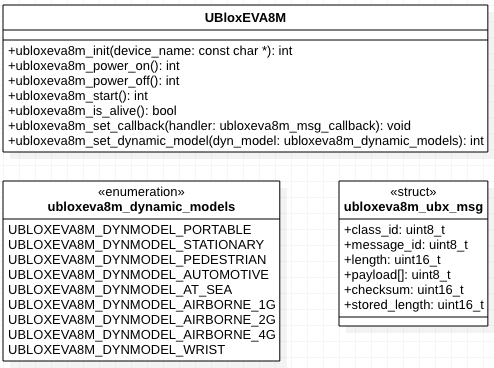
\includegraphics[width=0.8\columnwidth]{driver_ubloxeva8m_uml.png} 
\caption{Diagramme de class du driver UBloxEVA8M}
\label{fig:driver_ubloxeva8m_uml}
\end{figure}

Un exemple d'utilisation du driver UBloxEVA8M est proposée ci-dessous. Le principe d'utilisation et la configuration d'une fonction qui est appelé par le driver lorsqu'un nouveau message est reçu, une fonction callback. Dans cette fonction, l'utilisateur peut vérifier de quel type de message il s'agit, dans le cas ou le message l'intéresse il peut ensuite utiliser les structures permettant le décodage des différents messages.

\begin{lstlisting}[style=CStyle]
#include "UBloxEVA8M.h"

/* Function to print a UBX-NAV-PVT message */
static void print_nav_pvt_msg(char *txt, ubloxeva8m_nav_pvt_t* msg) {
	DBG_PRINTK("UBX-NAV-PVT: %d.%d.%d %02d:%02d:%02d:%03d validity=%d fixType=%d numSV=%d lat=%d lon=%d \n", msg->day, msg->month, msg->year, msg->hour, msg->minute, msg->seconds, msg->nano, msg->valid, msg->fixType, msg->numSV, msg->lat, msg->lon);
}

/* Callback function on GPS message */
static void gps_msg_callback(ubloxeva8m_ubx_msg* msg)
{
	ubloxeva8m_nav_pvt_t pvt_msg;
	
	/* Check message type */
	if (msg->class_id == UBLOXEVA8M_CLASS_NAV && msg->message_id == UBLOXEVA8M_MSG_NAV_PVT) {
		/* Copy message in struct */
		memcpy(&pvt_msg, msg->payload, sizeof(ubloxeva8m_nav_pvt_t));
		print_nav_pvt_msg("UBX-NAV-PVT: ", &pvt_msg);
	}
}

void main(void)
{
	int err;

	/* Initialize the gps */
	err = ubloxeva8m_init(CONFIG_I2C_SAM0_SERCOM3_LABEL);
	if (err) {
		DBG_PRINTK("%s: Can't initialize UBloxEVA8M %d\n", __func__, err);
		return;
	}

	/* Set callback function */
	ubloxeva8m_set_callback(gps_msg_callback);

	/* Start module */
	err = ubloxeva8m_start();
	if (err) {
		DBG_PRINTK("%s: Can't start GPS module %d\n", __func__, err);
		return;
	}

	/* Set the dynamic model used by the GPS */
	err = ubloxeva8m_set_dynamic_model(UBLOXEVA8M_DYNMODEL_AUTOMOTIVE);
	if (err) {
		DBG_PRINTK("%s: Can't set dynamic model %d\n", __func__, err);
		return;
	}
}
\end{lstlisting}

\subsection{Driver LSM303AGR}

Le driver LSM303AGR est le moyen de communiquer avec le module accéléromètre et magnétomètre qui est connecté au bus $I^{2}C$. Dans le cadre du projet seule la partie qui gère l'accéléromètre a été développée puisque le magnétomètre n'est pas utilisé. Le composant est décrit en détail dans le datasheet associé \cite{lsm303agr-datasheet}.

Le composant LSM303AGR est configuré au travers d'une liste de registre, il est également possible de lire les différentes valeurs mesurer au travers d'un autre groupe de registre. Tout les registres disponible sont détaillés dans le document \cite[p.~43]{lsm303agr-datasheet}.

Puisque le composant LSM303AGR se trouve placé sur le bus $I^{2}C$, ce driver utilise également le driver pour ce bus afin de pouvoir communiquer avec le module. La majorité des opérations consiste à écrire ou lire des valeurs dans les différents registres à disposition afin de configurer ou de récupérer les données voulues. Il est à noté qu'il est également possible de configurer le module afin qu'il produise des interruptions lorsque certains seuils sont dépassés sur un certain axe. Cette fonctionnalité est utilisé afin de détecter les pas effectuer par le porteur de capteur.

\todo{Revoir diagramme après implémentation finale}

La figure \ref{fig:driver_lsm303agr_uml} présente le diagramme de classe du driver LSM303AGR.

\begin{figure}[htb]
\centering 
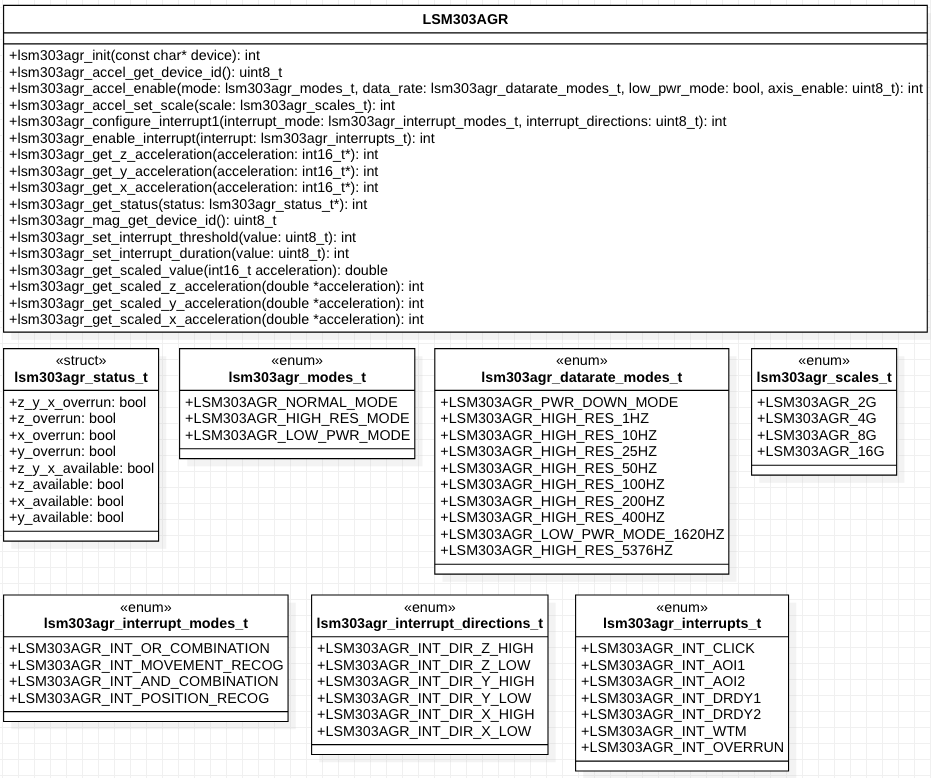
\includegraphics[width=1\columnwidth]{driver_lsm303agr_uml.png} 
\caption{Diagramme de class du driver LSM303AGR}
\label{fig:driver_lsm303agr_uml}
\end{figure}

Un exemple d'utilisation du driver est proposée ci-dessous.

\begin{lstlisting}[style=CStyle]
#include "LSM303AGR.h"

void main(void)
{
	int err;
	lsm303agr_status_t lsm_status;
	int16_t accel_x;
	int16_t accel_y;
	int16_t accel_z;

	/* Initialize the LSM303AGR module */
	err = lsm303agr_init(CONFIG_I2C_SAM0_SERCOM3_LABEL);
	if (err) {
		DBG_PRINTK("%s: Can't init LSM303AGR %d\n", __func__, err);
		return;
	}

	/* Enable the accelerometer */
	err = lsm303agr_accel_enable(LSM303AGR_NORMAL_MODE, LSM303AGR_HIGH_RES_100HZ, false, (LSM303AGR_Z_AXIS | LSM303AGR_Y_AXIS | LSM303AGR_X_AXIS));
	if (err) {
		DBG_PRINTK("%s: Can't enable accelerometer %d\n", __func__, err);
		return;
	}

	/* Set accelerometer scale */
	if (lsm303agr_accel_set_scale(LSM303AGR_8G)) {
		DBG_PRINTK("Couldn't set accelerometer scale\n");
		return;
	}
	
	/* Get accelerometer status */
	if (lsm303agr_get_status(&lsm_status)) {
		DBG_PRINTK("Couldn't get status\n");
		return;	
	}
	
	/* Get current acceleration on x axis */	
	if (lsm303agr_get_x_acceleration(&accel_x)) {
		DBG_PRINTK("Couldn't get acceleration\n");
		return;		
	}

	/* Get current acceleration on y axis */	
	if (lsm303agr_get_y_acceleration(&accel_y)) {
		DBG_PRINTK("Couldn't get acceleration\n");
		return;		
	}
	
	/* Get current acceleration on z axis */	
	if (lsm303agr_get_z_acceleration(&accel_z)) {
		DBG_PRINTK("Couldn't get acceleration\n");
		return;		
	}	
}
\end{lstlisting}

\todo{Add setup of IRQ}

\subsection{Driver RN2483}

Le driver RN2483 permet de piloter le composant du même nom qui permet la communication radio LoRa. Le module est connecté au micro-contrôleur par un UART et il est piloté grâce à un protocole de commande texte qui permette d'effectuer les différentes opérations requises pour l'envoie de donnée.

Le protocole est détaillé dans le document Command Reference User's Guide \cite{rn2483-datasheet}.

Grâce au driver il est possible à l'utilisateur d'effectuer certaines opérations, le driver se charge de créer les bonnes commandes et de les envoyer sur l'UART. Une fois la commande exécutée par le module il vérifie également le bon acquittement de celle-ci.

Il est aussi possible de gérer la couche MAC LoRaWAN grâce au composant, puisque cette couche n'est pas utilisée dans le cadre du projet, elle est désactivée au moyen de la fonction rn2483\_lora\_pause\_mac() et seule la couche radio LoRa est utilisée pour envoyer des messages, cela permet de simplifier grandement la gestion du protocole de communication.

La figure \ref{fig:driver_rn2483_uml} présente le diagramme de classe du driver RN2483.

\begin{figure}[htb]
\centering 
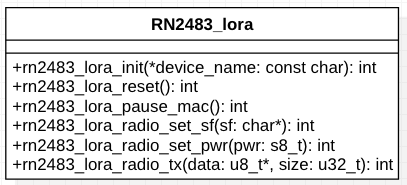
\includegraphics[width=0.6\columnwidth]{driver_rn2483_uml.png} 
\caption{Diagramme de class du driver RN2483}
\label{fig:driver_rn2483_uml}
\end{figure}

Un exemple d'utilisation du driver est proposée ci-dessous.

\begin{lstlisting}[style=CStyle]
#include "RN2483.h"

/**
 * LoRa spreading factor
 * (Between sf7 and sf12)
 */
#define LORA_SPREADING_FACTOR "sf7"

/**
 * LoRa power output
 */
#define LORA_POWER_OUTPUT 1

#define BUFFER_SIZE 56

void main(void)
{
	int err;
	u8_t buffer[BUFFER_SIZE];

	/* Initialize the UART */
	err = rn2483_lora_init(CONFIG_UART_SAM0_SERCOM2_LABEL);
	if (err) {
		DBG_PRINTK("%s: Can't init RN2483 %d\n", __func__, err);
		return;
	}

	/* Pause mac layer */
	err = rn2483_lora_pause_mac();
	if (err) {
		DBG_PRINTK("%s: Can't pause mac layer %d\n", __func__, err);
		return;
	}

	/* Set spreading factor */
	err = rn2483_lora_radio_set_sf(LORA_SPREADING_FACTOR);
	if (err) {
		DBG_PRINTK("%s: Can't set spreading factor %d\n", __func__, err);
		return;
	}

	/* Set power output */
	err = rn2483_lora_radio_set_pwr(LORA_POWER_OUTPUT);
	if (err) {
		DBG_PRINTK("%s: Can't set power output %d\n", __func__, err);
		return;
	}
	
	/* Send data */
	buffer[0] = 0x11;
	buffer[1] = 0x22;
	buffer[2] = 0x33;
	buffer[3] = 0x44;
	
	if (rn2483_lora_radio_tx(buffer, 4) {
		DBG_PRINTK("Couldn't send packet\n");
		return;
	}	
}
\end{lstlisting}

\subsection{Driver LEDs}

La carte SODAQ One est équipée de 3 LEDs, une rouge, une verte, une bleu, qui sont connectés à des GPIOs. Ce driver, très simple, permet d'abstraire la gestion des GPIO et propose une interface facilitant la gestion des LEDs.

La figure \ref{fig:driver_led_uml} présente le diagramme de classe du driver LED.

\begin{figure}[htb]
\centering 
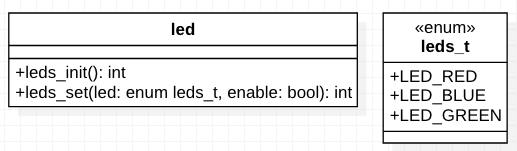
\includegraphics[width=0.6\columnwidth]{driver_led_uml.png} 
\caption{Diagramme de class du driver LED}
\label{fig:driver_led_uml}
\end{figure}

Un exemple d'utilisation du driver est disponible ci-dessous.

\begin{lstlisting}[style=CStyle]
#include "led.h"

void main(void)
{
	int err;

	err = leds_init();
	if (err) {
		DBG_PRINTK("%s: Cannot initialize LEDs\n", __func__);
		return;
	}
	
	while(1) {
		/* Switch-on LED */
		leds_set(LED_RED, true);
		/* Delay */
		k_sleep(K_SECONDS(1));
		/* Switch-off LED */
		leds_set(LED_RED, false);
		/* Delay */
		k_sleep(K_SECONDS(1));		
	}
}
\end{lstlisting}

\subsection{Driver External Interrupt Controller}

Lorsqu'un battement du cœur du sportif est détecté par le module rythme cardiaque, une impulsion est générée sur une ligne connectée à un GPIO du micro-contrôleur. Afin de pouvoir compter proprement les battements une interruption doit pouvoir être déclenchée lorsque l'impulsion est détectée. Dans Zephyr cela se traduit par la configuration au travers du driver GPIO, on peut spécifier si l'on souhaite déclencher une interruption et dans quelles conditions, flanc montant ou descendant ou alors lors d'un niveau haut ou bas. Cependant cette fonctionnalité n'était pas présente au moment du travail de Bachelor. Afin de pouvoir proposer cette fonctionnalité un driver de gestion des interruptions externe ou External Interrupt Controller (EIC) a du être développé. Une fois le driver développé il a fallut ensuite modifier le driver GPIO afin de pouvoir proposer cette fonctionnalité.

La figure \ref{fig:driver_eic_uml} présente le diagramme de classe du driver External Interrupt Controller.

\begin{figure}[htb]
\centering 
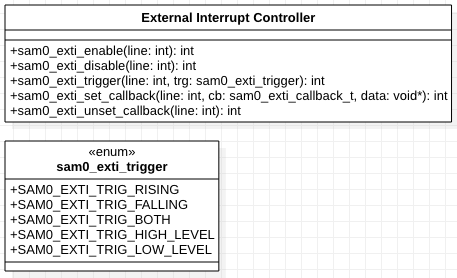
\includegraphics[width=0.6\columnwidth]{eic_uml.png} 
\caption{Diagramme de class du driver External Interrupt Controller}
\label{fig:driver_eic_uml}
\end{figure}

Un exemple d'utilisation du driver est disponible ci-dessous.

\begin{lstlisting}[style=CStyle]
#include "exti_sam0.h"

void gpio_callback(int line, void *user)
{
	DBG_PRINTK("GPIO interruption triggered");
}

void main(void)
{
	int err;
	int line = 1;

	err = sam0_exti_enable(line);
	if (err) {
		DBG_PRINTK("%s: Cannot enable external interrupt\n", __func__);
		return;	
	}
	
	err = sam0_exti_trigger(line, SAM0_EXTI_TRIG_RISING);
	if (err) {
		DBG_PRINTK("%s: Cannot set interrupt trigger type\n", __func__);
		return;	
	}

	err = sam0_exti_set_callback(line , gpio_callback);
	if (err) {
		DBG_PRINTK("%s: Cannot set interrupt trigger type\n", __func__);
		return;	
	}	

	while (1) {
		k_sleep(K_SECONDS(1));	
	}
}
\end{lstlisting}


\section{Paquet de donnée}

Le capteur transmet les données qui sont acquises au cours de la course grâce à un paquet de donnée LoRa. Le format et le contenu de ce paquet sont présentés ci-dessous.

\begin{figure}[htb]
\centering 
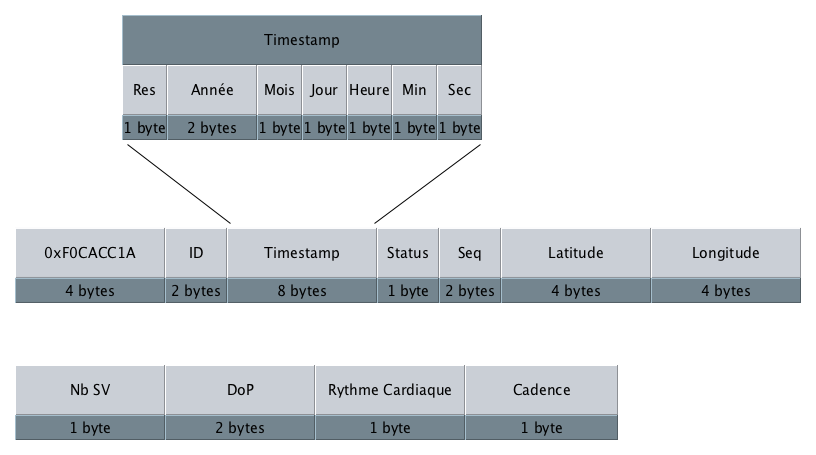
\includegraphics[width=1\columnwidth]{sensor_packet_format.png} 
\caption{Format du paquet de donnée LoRa}
\label{fig:sensor_packet_format}
\end{figure}

Le paquet fait une taille totale de 30 bytes et est composé des éléments suivants.

\begin{table}[htb]
\caption{Détails des champs du paquet de données radio LoRa}
\label{tab:sensor_packet_format}
\centering
\begin{tabular}{ l l l p{9cm} l }
\toprule
Champs & Taille & Type & Description \\
\midrule
Marqueur & 4 & uint & Une valeur fixe servant de marqueur et permettant d'identifier que le paquet provient bien d'un capteur du système \\
ID & 1 & uint & Identifiant du capteur qui a généré le paquet \\
Timestamp & 8 & uint & Heure et date au moment de la génération du paquet \\
Status & 1 & uint & Status du capteur \\
Seq & 1 & uint & Numéro de séquence du paquet. Chaque fois qu'un paquet est généré le compteur est incrémenté de un, cela permet de détecter lorsque des paquets sont perdu \\
Latitude & 4 & int & Latitude du capteur reporté directement depuis le module GPS \\
Longitude & 4 & int & Longitude du capteur reporté directement depuis le module GPS \\
Nb SV & 1 & uint & Nombre de satellites GPS en vue \\
DoP & 2 & int & Disolution of Position, la qualité de la précision de la position GPS \\
Rythme cardiaque & 1 & uint & Rythme cardiaque de l'athlète \\
Cadence & 1 & uint & Cadence de l'athlète \\
\bottomrule 
\end{tabular}
\end{table}

\section{Le débuggage}

\todo{}

\section{Le boîtier}

\todo{}
